%%%%%%%%%%%%%%%%%%%%%%%%%%%%%%%%%%%%%%%%%%%%%%%%%%%%%%
\newpage
\pagestyle{fancy}

\chapter{Title of the Chapter 5}
\minitoc
\newpage
\label{chap.5}

\section{Cellario} \label{chap5:sec1}

\subsection{Full vs cut stent}
Bulge pressure on the full stent:

\begin{figure}[ht]
	\centering
	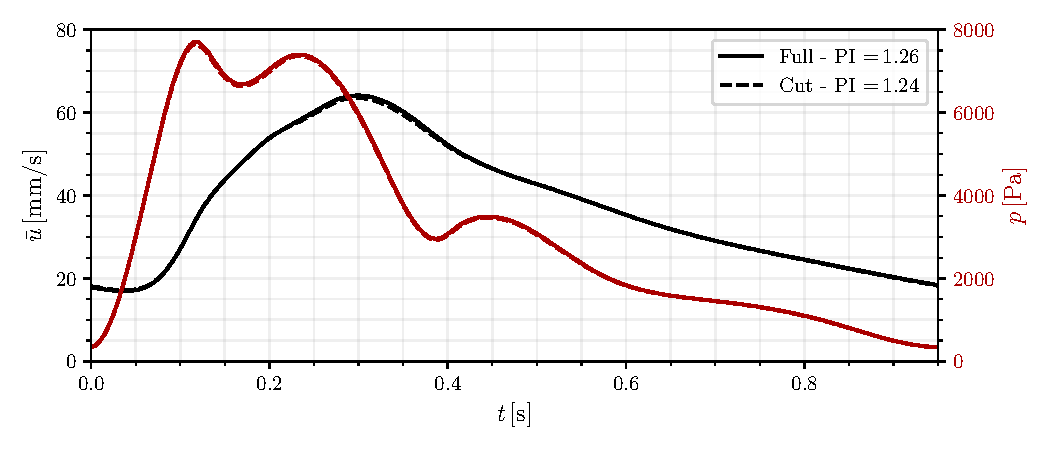
\includegraphics[width=\textwidth]{chapter5/Figures/Convergence/cut_full_comparison.pdf}
	\renewcommand{\arraystretch}{1.4}
	\setlength{\tabcolsep}{10pt}
	\begin{tabular}{cccccc}
		\toprule
		\multicolumn{2}{c}{\textbf{Comparison}} & \textbf{Mean}     & \textbf{Std} & \textbf{Min} & \textbf{Max}           \\
		\midrule
		\multirow{2}{*}{Full stent}             & $p\,$[\pa]        & 3257.65      & 2376.46      & 337.604      & 7708.38 \\
		                                        & $\bar{u}$\,[mm/s] & 37.5429      & 14.8827      & 16.9161      & 64.1167 \\
		\midrule
		\multirow{2}{*}{Cut stent}              & $p\,$[\pa]        & 3236.66      & 2361.91      & 333.288      & 7653.89 \\
		                                        & $\bar{u}$\,[mm/s] & 37.4279      & 14.7269      & 17.1103      & 63.5877 \\
		\bottomrule
	\end{tabular}
	\caption[Comparison between cut and full stents]{Comparison between the hemodynamics of using a full stent section and using a stent reduced to the areas exposed to neck and branches. The variables considered are the intra-aneurysmal velocity magnitude $\bar{u}$ (black), the pressure (red) and the Pulsatility Index (PI) given in the legend. These quantities are integrated over the aneurysm sack and normalized by the sack volume.}\label{fig:fullvscut}
\end{figure}

\begin{equation}
	\text{PI} = \frac{\max(\bar{u}) - \min(\bar{u})}{\text{mean}(\bar{u})}
\end{equation}


\section{Second Section}\label{chap5:sec2}

\section{Third Section}\label{chap5:sec3}

\bibliographystyle{elsarticle-num}
\bibliography{chapter5/Biblio}